\documentclass{beamer}

\usepackage{adjustbox}
\usepackage{listings}
\usepackage{graphicx}
\usepackage{mathtools}
\usepackage{tikz}
\usepackage[T1]{fontenc}

\usetikzlibrary{calc,trees,positioning,arrows,chains,shapes.geometric,%
                decorations.pathreplacing,decorations.pathmorphing,shapes,%
                matrix,shapes.symbols,fit,scopes}

\tikzset{
    >=stealth',
    punktchain/.style={
        rectangle,
        rounded corners,
        draw=black, very thick,
        text width=10em,
        minimum height=3em,
        text centered,
        on chain
    },
    line/.style={draw, thick, <-},
    element/.style={
        tape,
        top color=white,
        bottom color=blue!50!black!60!,
        minimum width=8em,
        draw=blue!40!black!90, very thick,
        text width=10em,
        minimum height=3.5em,
        text centered,
        on chain
    },
    every join/.style={->, thick, shorten >=1pt},
    decoration={brace},
    tuborg/.style={decorate},
    tubnode/.style={midway, right=2pt},
    llchain/.style={
        rectangle,
        rounded corners,
        draw=black, very thick,
        text width=2em,
        minimum height=3em,
        text centered,
        on chain
    }
}

\begin{document}
    \title{Demystifying Haskell}
    \subtitle{An in-depth examination of the Fibonacci sequence.}
    \author{Andrew Rademacher}

    \definecolor{dkgreen}{rgb}{0,0.6,0}
    \definecolor{gray}{rgb}{0.5,0.5,0.5}
    \definecolor{mauve}{rgb}{0.58,0,0.82}

    \lstdefinelanguage{JavaScript}{
        keywords={typeof, new, true, false, catch, function, return, null, catch, switch, var, if, in, while, do, else, case, break},
        keywordstyle=\color{blue}\bfseries,
        ndkeywords={class, export, boolean, throw, implements, import, this},
        ndkeywordstyle=\color{darkgray}\bfseries,
        identifierstyle=\color{black},
        sensitive=false,
        comment=[l]{//},
        morecomment=[s]{/*}{*/},
        commentstyle=\color{purple}\ttfamily,
        stringstyle=\color{red}\ttfamily,
        morestring=[b]',
        morestring=[b]"
    }

    \lstset{
        frame=tb,
        basicstyle=\ttfamily,
        columns=flexible,
        breaklines=true,
        breakatwhitespace=true,
        aboveskip=3mm,
        belowskip=3mm,
        showstringspaces=false,
        numbers=left,
        numberstyle=\tiny\color{gray},
        keywordstyle=\color{blue},
        commentstyle=\color{dkgreen},
        stringstyle=\color{mauve},
        tabsize=3
    }

% FRAME:TITLE
    \frame{\titlepage}

% FRAME:FIBONACCI
    \begin{frame}
        \frametitle{The Fibonacci Sequence}

        \begin{columns}[c]
            \begin{column}[T]{5cm}
                \begin{itemize}
                    \item Sequence is infinite
                    \item Sequence is self-referencing
                    \item Values grow exponentially
                    \item Values are always positive
                \end{itemize}
            \end{column}
            \begin{column}[T]{5cm}
                \begin{figure}
                    \centering
                    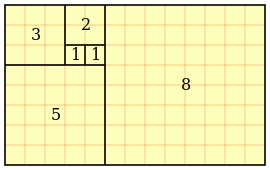
\includegraphics[height=3cm]{./images/FibonacciBlocks.png}
                \end{figure}

                \begin{figure}
                    \centering
                    \begin{math}
                        \left\{1,1,2,3,5,8...\right\}
                    \end{math}
                \end{figure}
               
                \begin{figure}
                    \centering
                    \begin{math}
                        F_{n} = F_{n-1} + F_{n-2}
                    \end{math}
                \end{figure}
            \end{column}
        \end{columns}
    \end{frame}

% FRAME:JAVASCRIPT
    \lstset{language=JavaScript}
    \begin{frame}[fragile=singleslide]
        \frametitle{Traditional JavaScript Implementation}

        \begin{lstlisting}
function getFibs (n) {
    var fibs = [1, 1];
    for (var i = 2; i < n; i++) 
        fibs.push(fibs[fibs.length - 1] + fibs[fibs.length - 2]);

    return fibs;
}
        \end{lstlisting}
    \end{frame}

% FRAME:JAVA
    \lstset{language=Java}
    \begin{frame}[fragile=singleslide]
        \frametitle{Traditional Java Implementation}
        
        \begin{lstlisting}
public static BigInteger[] getFibs(int n) {
    BigInteger[] fibs = new BigInteger[n];
    fibs[0] = BigInteger.valueOf(1);
    fibs[1] = BigInteger.valueOf(1);
    for (int i = 2; i < n; i++)
        fibs[i] = fibs[i - 1].add(fibs[i - 2]);

    return fibs;
}
        \end{lstlisting}
    \end{frame}

% FRAME:PROCESS
    \begin{frame}[fragile=singleslide]
        \frametitle{Imperative Process}
        
        \adjustbox{scale=0.5}{
            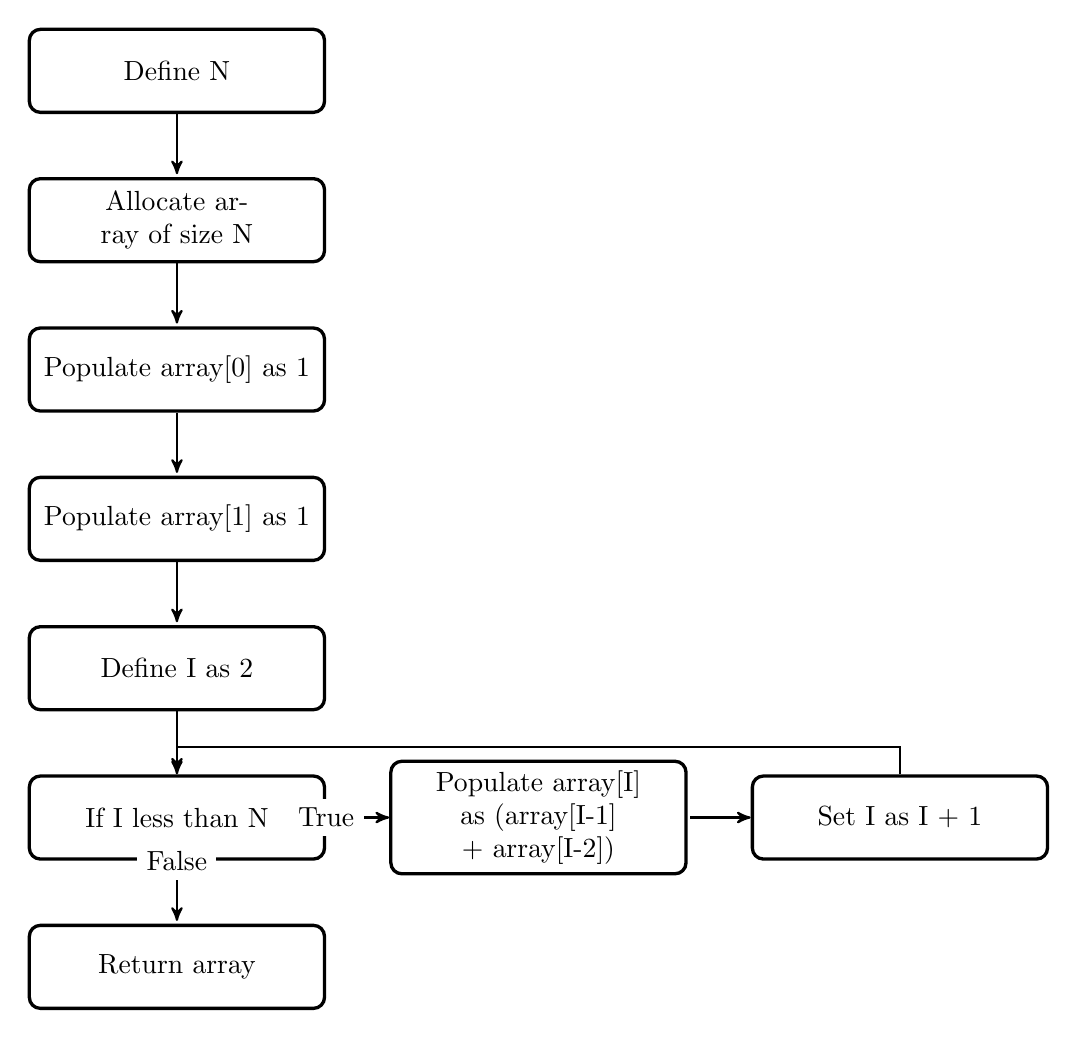
\begin{tikzpicture}[node distance=0.8cm,start chain=going below]
                \node[punktchain, join] (defineN) {Define N};
                \node[punktchain, join] (alloc) {Allocate array of size N};
                \node[punktchain, join] (pop0) {Populate array[0] as 1};
                \node[punktchain, join] (pop1) {Populate array[1] as 1};
                \node[punktchain, join] (defineI) {Define I as 2};
                
                \node[punktchain, join] (if) {If I less than N};
                \begin{scope}[start branch=venstre, every join/.style={->, thick, shorten <=1pt}]
                    \node[punktchain, on chain=going right, join=by {->}] 
                        (popI) {Populate array[I] as (array[I-1] + array[I-2])};
                    \node[punktchain, on chain=going right, join=by {->}]
                        (setI) {Set I as I + 1};
                \end{scope}
                
                \node[punktchain, join] (return) {Return array};

                % -- Post processing -- %

                \draw (if.east) node [fill=white] {True};
                \draw[|-,-|,->,thick] (setI.north) |-+(0,1em)-| (if.north);
                \draw (if.south) node [fill=white] {False};
            \end{tikzpicture}
        }
    \end{frame}

% FRAME:HASKELL
    \lstset{language=Haskell}
    \begin{frame}[fragile=singleslide]
        \frametitle{New Fangled Haskell Implementation}

        \begin{lstlisting}
fibs = 1 : 1 : [ a + b | (a, b) <- zip fibs (tail fibs) ]
        \end{lstlisting}
    \end{frame}

% FRAME:WHAT
    \begin{frame}[fragile=singleslide]
        \begin{figure}
            \centering
            
\includegraphics[scale=0.35]{./images/lolwutpear.jpg}
        \end{figure}
    \end{frame}

% FRAME:ASSIGNMENT
    \lstset{language=Haskell}
    \begin{frame}[fragile=singleslide]
        \frametitle{Values != Variables}

        \begin{columns}[c]
            \begin{column}[T]{5cm}
                \begin{itemize}
                    \item Haskell has no variables
                    \item Values can be bound to a name
                    \item Values can only be assigned once
                    \item Values never change
                \end{itemize}
            \end{column}
            \begin{column}[T]{5cm}
                \begin{lstlisting}
fibs = 1 // Valid assignment
fibs = 2 // Invalid assignment
                \end{lstlisting}
            \end{column}
        \end{columns}
    \end{frame}

% FRAME:LISTS
    \begin{frame}[fragile=singleslide]
        \frametitle{Lists}

        \begin{columns}[c]
            \begin{column}[T]{5cm}
                \begin{itemize}
                    \item Lists are singly-linked
                    \item Lists are homogeneous
                    \item Lists are immutable
                    \item Lists use head insertion
                    \item Two lists can share structure
                \end{itemize}
            \end{column}
            \begin{column}[T]{5cm}
                \begin{figure}
                    \centering
                    \adjustbox{scale=0.5} {
                        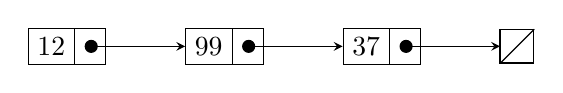
\begin{tikzpicture}[list/.style={rectangle split, rectangle split parts=2, draw, rectangle split horizontal}, >=stealth, start chain]
                            \node[list,on chain] (A) {12};
                            \node[list,on chain] (B) {99};
                            \node[list,on chain] (C) {37};
                            \node[on chain,draw,inner sep=6pt] (D) {};
                            \draw (D.north east) -- (D.south west);
                            \draw (D.north west) -- (D.south west);
                            \draw[*->] let \p1 = (A.two), \p2 = (A.center) in (\x1,\y2) -- (B);
                            \draw[*->] let \p1 = (B.two), \p2 = (B.center) in (\x1,\y2) -- (C);
                            \draw[*->] let \p1 = (C.two), \p2 = (C.center) in (\x1,\y2) -- (D);
                        \end{tikzpicture}
                    }
                    \adjustbox{scale=0.5} {
                        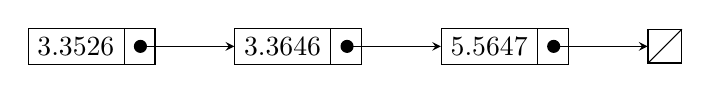
\begin{tikzpicture}[list/.style={rectangle split, rectangle split parts=2, draw, rectangle split horizontal}, >=stealth, start chain]
                            \node[list,on chain] (A) {3.3526};
                            \node[list,on chain] (B) {3.3646};
                            \node[list,on chain] (C) {5.5647};
                            \node[on chain,draw,inner sep=6pt] (D) {};
                            \draw (D.north east) -- (D.south west);
                            \draw (D.north west) -- (D.south west);
                            \draw[*->] let \p1 = (A.two), \p2 = (A.center) in (\x1,\y2) -- (B);
                            \draw[*->] let \p1 = (B.two), \p2 = (B.center) in (\x1,\y2) -- (C);
                            \draw[*->] let \p1 = (C.two), \p2 = (C.center) in (\x1,\y2) -- (D);
                        \end{tikzpicture}
                    }
                    \adjustbox{scale=0.5} {
                        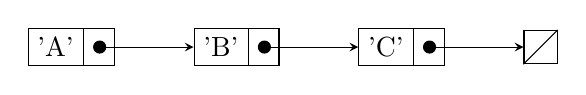
\begin{tikzpicture}[list/.style={rectangle split, rectangle split parts=2, draw, rectangle split horizontal}, >=stealth, start chain]
                            \node[list,on chain] (A) {'A'};
                            \node[list,on chain] (B) {'B'};
                            \node[list,on chain] (C) {'C'};
                            \node[on chain,draw,inner sep=6pt] (D) {};
                            \draw (D.north east) -- (D.south west);
                            \draw (D.north west) -- (D.south west);
                            \draw[*->] let \p1 = (A.two), \p2 = (A.center) in (\x1,\y2) -- (B);
                            \draw[*->] let \p1 = (B.two), \p2 = (B.center) in (\x1,\y2) -- (C);
                            \draw[*->] let \p1 = (C.two), \p2 = (C.center) in (\x1,\y2) -- (D);
                        \end{tikzpicture}
                    }
                    \caption{Haskell Lists}
                \end{figure}
                \begin{figure}
                    \adjustbox{scale=0.5} {
                        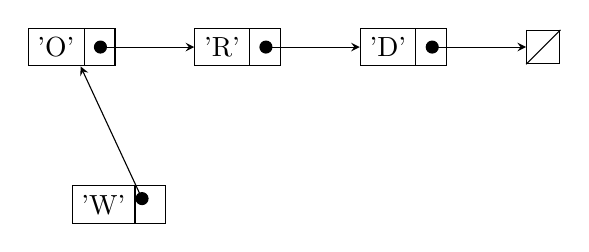
\begin{tikzpicture}[list/.style={rectangle split, rectangle split parts=2, draw, rectangle split horizontal}, >=stealth, start chain]
                            \node[list,on chain] (A) {'O'};
                            \node[list,on chain] (B) {'R'};
                            \node[list,on chain] (C) {'D'};
                            \node[on chain,draw,inner sep=6pt] (D) {};
                            \draw (D.north east) -- (D.south west);
                            \draw (D.north west) -- (D.south west);
                            \draw[*->] let \p1 = (A.two), \p2 = (A.center) in (\x1,\y2) -- (B);
                            \draw[*->] let \p1 = (B.two), \p2 = (B.center) in (\x1,\y2) -- (C);
                            \draw[*->] let \p1 = (C.two), \p2 = (C.center) in (\x1,\y2) -- (D);

                            \node[list,on chain] (E) at (-1,-2) {'W'};
                            \draw[*->] let \p1 = (E.two), \p2 = (E.center) in (\x1,\y2) -- (A);
                        \end{tikzpicture}
                    }
                    \caption{List Insertion}
                \end{figure}
            \end{column}
        \end{columns}
    \end{frame}

% FRAME:LIST OPERATIONS
    \begin{frame}[fragile=singleslide]
        \frametitle{Basic List Operations}

        \begin{lstlisting}
listA = [1, 2, 3, 4, 5]             // Literal
listB = [6, 7, 8]                   // Literal

listC = listA ++ listB              // Concatenation
// listC = [1, 2, 3, 4, 5, 6, 7, 8]

listD = 0 : listC                   // Insert
// listD = [0, 1, 2, 3, 4, 5, 6, 7, 8]
        \end{lstlisting}
    \end{frame}

% FRAME:LIST FUNCTIONS
    \begin{frame}[fragile=singleslide]
        \frametitle{List Functions}

        \begin{columns}[c]
            \begin{column}[T]{5cm}
                \begin{description}
                    \item[head] \hfill \\
                        The first element in a list.
                    \item[tail] \hfill \\
                        All remaining elements in a list.
                \end{description}
            \end{column}
            \begin{column}[T]{5cm}
                \begin{figure}
                    \adjustbox{scale=0.5} {
                        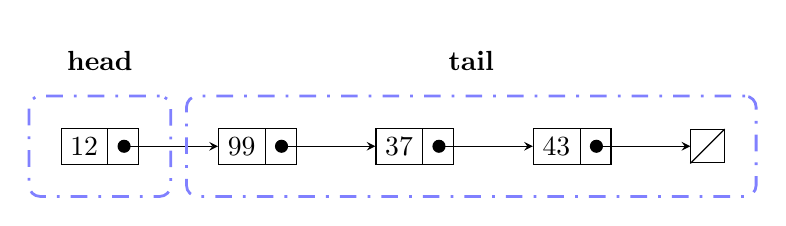
\begin{tikzpicture}[list/.style={rectangle split, rectangle split parts=2, draw, rectangle split horizontal}, >=stealth, start chain]
                            \node[list,on chain] (A) {12};
                            \node[list,on chain] (B) {99};
                            \node[list,on chain] (C) {37};
                            \node[list,on chain] (D) {43};
                            \node[on chain,draw,inner sep=6pt] (E) {};
                            \draw (E.north east) -- (E.south west);
                            \draw (E.north west) -- (E.south west);
                            \draw[*->] let \p1 = (A.two), \p2 = (A.center) in (\x1,\y2) -- (B);
                            \draw[*->] let \p1 = (B.two), \p2 = (B.center) in (\x1,\y2) -- (C);
                            \draw[*->] let \p1 = (C.two), \p2 = (C.center) in (\x1,\y2) -- (D);
                            \draw[*->] let \p1 = (D.two), \p2 = (D.center) in (\x1,\y2) -- (E);

                            \tikzset{blue dotted/.style={draw=blue!50!white, line width=1pt,
                                        dash pattern=on 1pt off 4pt on 6pt off 4pt,
                                        inner sep=4mm, rectangle, rounded corners}};

                            \node (first dotted box) [blue dotted, 
                                                        fit = (A) ] {};
                            \node (second dotted box) [blue dotted,
                                                        fit = (B) (E)] {};

                            \node at (first dotted box.north) [above, inner sep=3mm] {\textbf{head}};
                            \node at (second dotted box.north) [above, inner sep=3mm] {\textbf{tail}};

                        \end{tikzpicture}
                    }
                \end{figure}
                \begin{figure}
                    \begin{lstlisting}
listA = [1, 2, 3, 4]

headA = head listA
//  headA = 1
tailA = tail listA
//  tailA = [2, 3, 4]
                    \end{lstlisting}
                \end{figure}
            \end{column}
        \end{columns}
    \end{frame}

% FRAME:TUPLES
    \begin{frame}[fragile=singleslide]
        \frametitle{Tuples}

        \begin{columns}[c]
            \begin{column}[T]{5cm}
                \begin{itemize}
                    \item Tuples are atomic (like an int or boolean).
                    \item Tuples are heterogeneous.
                    \item Tuples are immutable.
                    \item Tuples allow random access.
                    \item Tuples are usually small (less than 4 elements).
                \end{itemize}
            \end{column}
            \begin{column}[T]{5cm}
                \begin{lstlisting}
coord  = 
    (23.235, -345.345)
name   = 
    ("John", "Edward", "Doe")
person = 
    ("Jane Doe", 24, Female)
complex =
    ("SGF", [2,3,4], [2.3,2.5])
                \end{lstlisting}
            \end{column}
        \end{columns}
    \end{frame}

% FRAME:ZIP FUNCTION (1)
    \begin{frame}[fragile=singleslide]
        \frametitle{Zip (Lists and Tuples)}

        \adjustbox{scale=0.7} {
            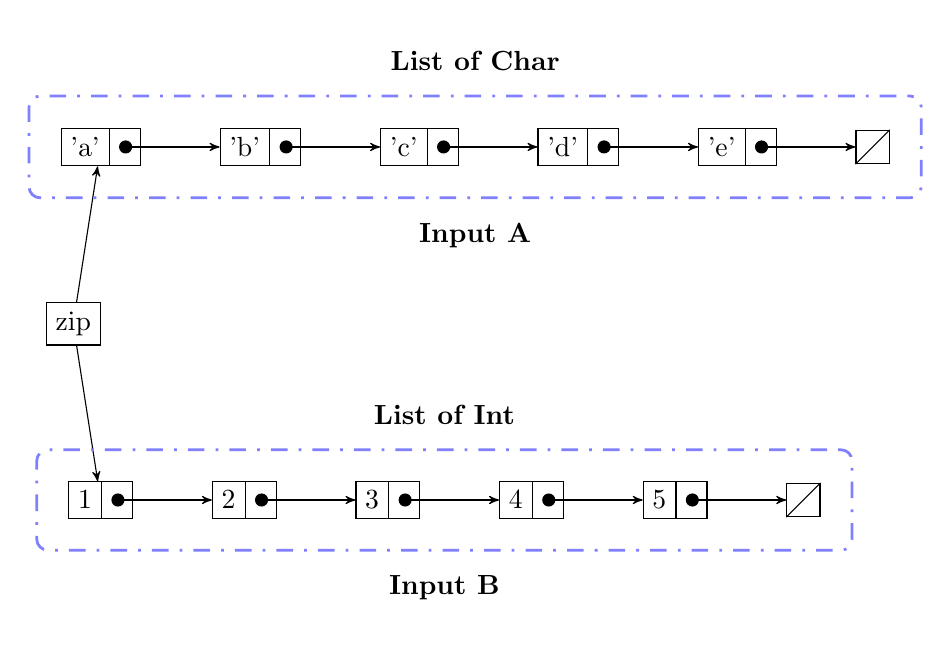
\begin{tikzpicture}[
            list/.style={
                rectangle split,
                rectangle split parts=2,
                draw,
                rectangle split horizontal
            },
            blue dotted/.style={
                draw=blue!50!white,
                line width=1pt,
                dash pattern=on 1pt off 4pt on 6pt off 4pt,
                inner sep=4mm,
                rectangle,
                rounded corners
            },
            node distance=2mm and 1cm]
                { [start chain=zip]
                    \node[on chain,draw,rectangle] (zip) {zip};
                    { [start branch=letters going right]
                        \node[list,on chain, above=2cm] (B1) {'a'};
                        \node[list,on chain] (B2) {'b'};
                        \node[list,on chain] (B3) {'c'};
                        \node[list,on chain] (B4) {'d'};
                        \node[list,on chain] (B5) {'e'};
                        \node[on chain,draw,inner sep=6pt] (B6) {};
                   
                        \draw (B6.north east) -- (B6.south west);
                        \draw[*->] let \p1 = (B1.two), \p2 = (B1.center) in (\x1,\y2) -- (B2);
                        \draw[*->] let \p1 = (B2.two), \p2 = (B2.center) in (\x1,\y2) -- (B3);
                        \draw[*->] let \p1 = (B3.two), \p2 = (B3.center) in (\x1,\y2) -- (B4);
                        \draw[*->] let \p1 = (B4.two), \p2 = (B4.center) in (\x1,\y2) -- (B5);
                        \draw[*->] let \p1 = (B5.two), \p2 = (B5.center) in (\x1,\y2) -- (B6);
                        \draw[->] (zip) -- (B1);

                        \node (letters dotted box) [blue dotted, fit = (B1) (B6)] {};
                        \node at (letters dotted box.north) [above, inner sep=3mm] {\textbf{List of Char}};
                        \node at (letters dotted box.south) [below, inner sep=3mm] {\textbf{Input A}};
                    }
                    { [start branch=numbers going right]
                        \node[list,on chain, below=2cm] (C1) {1};
                        \node[list,on chain] (C2) {2};
                        \node[list,on chain] (C3) {3};
                        \node[list,on chain] (C4) {4};
                        \node[list,on chain] (C5) {5};
                        \node[on chain,draw,inner sep=6pt] (C6) {};
                        
                        \draw (C6.north east) -- (C6.south west);
                        \draw[*->] let \p1 = (C1.two), \p2 = (C1.center) in (\x1,\y2) -- (C2);
                        \draw[*->] let \p1 = (C2.two), \p2 = (C2.center) in (\x1,\y2) -- (C3);
                        \draw[*->] let \p1 = (C3.two), \p2 = (C3.center) in (\x1,\y2) -- (C4);
                        \draw[*->] let \p1 = (C4.two), \p2 = (C4.center) in (\x1,\y2) -- (C5);
                        \draw[*->] let \p1 = (C5.two), \p2 = (C5.center) in (\x1,\y2) -- (C6);
                        \draw[->] (zip) -- (C1);

                        \node (numbers dotted box) [blue dotted, fit = (C1) (C6)] {};
                        \node at (numbers dotted box.north) [above, inner sep=3mm] {\textbf{List of Int}};
                        \node at (numbers dotted box.south) [below, inner sep=3mm] {\textbf{Input B}};
                    }
                }
            \end{tikzpicture}
        }
    \end{frame}

% FRAME:ZIP FUNCTION (2)
    \begin{frame}[fragile=singleslide]
        \frametitle{Zip (Lists and Tuples)}

        \adjustbox{scale=0.7} {
            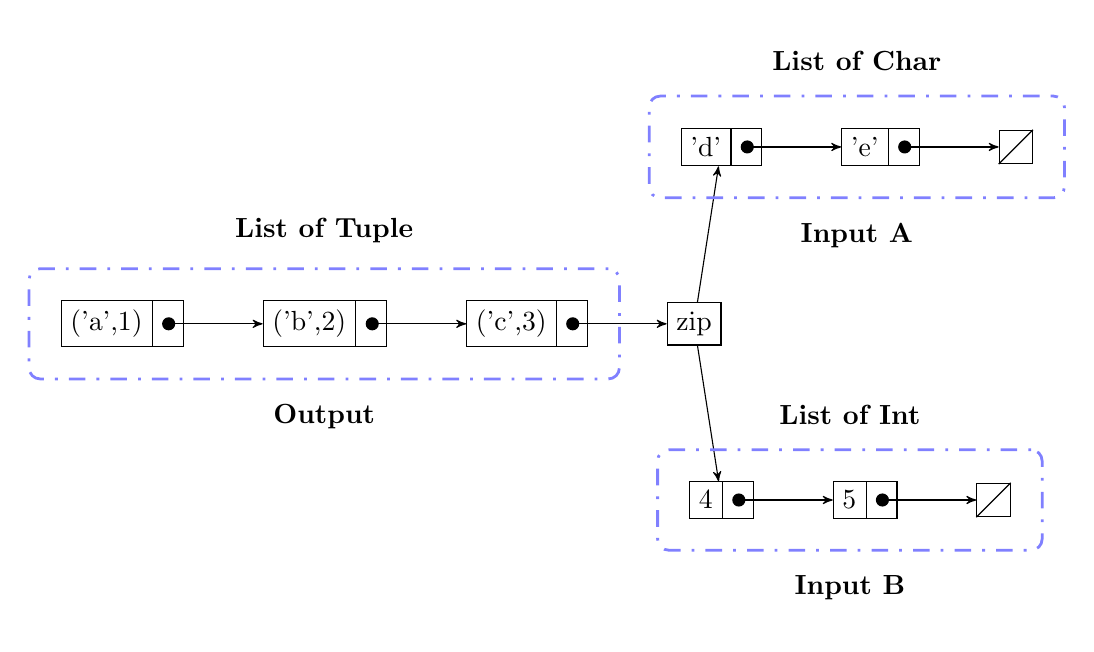
\begin{tikzpicture}[
            list/.style={
                rectangle split,
                rectangle split parts=2,
                draw,
                rectangle split horizontal
            },
            blue dotted/.style={
                draw=blue!50!white,
                line width=1pt,
                dash pattern=on 1pt off 4pt on 6pt off 4pt,
                inner sep=4mm,
                rectangle,
                rounded corners
            },
            node distance=2mm and 1cm]
                { [start chain=zip]
                    \node[list,on chain] (A1) {('a',1)};
                    \node[list,on chain] (A2) {('b',2)};
                    \node[list,on chain] (A3) {('c',3)};
                    \node[on chain,draw,rectangle] (zip) {zip};
                    { [start branch=letters going right]
                        \node[list,on chain, above=2cm] (B1) {'d'};
                        \node[list,on chain] (B2) {'e'};
                        \node[on chain,draw,inner sep=6pt] (B3) {};
                   
                        \draw (B3.north east) -- (B3.south west);
                        \draw[*->] let \p1 = (B1.two), \p2 = (B1.center) in (\x1,\y2) -- (B2);
                        \draw[*->] let \p1 = (B2.two), \p2 = (B2.center) in (\x1,\y2) -- (B3);
                        \draw[->] (zip) -- (B1);

                        \node (letters dotted box) [blue dotted, fit = (B1) (B3)] {};
                        \node at (letters dotted box.north) [above, inner sep=3mm] {\textbf{List of Char}};
                        \node at (letters dotted box.south) [below, inner sep=3mm] {\textbf{Input A}};
                    }
                    { [start branch=numbers going right]
                        \node[list,on chain, below=2cm] (C1) {4};
                        \node[list,on chain] (C2) {5};
                        \node[on chain,draw,inner sep=6pt] (C3) {};
                        
                        \draw (C3.north east) -- (C3.south west);
                        \draw[*->] let \p1 = (C1.two), \p2 = (C1.center) in (\x1,\y2) -- (C2);
                        \draw[*->] let \p1 = (C2.two), \p2 = (C2.center) in (\x1,\y2) -- (C3);
                        \draw[->] (zip) -- (C1);

                        \node (numbers dotted box) [blue dotted, fit = (C1) (C3)] {};
                        \node at (numbers dotted box.north) [above, inner sep=3mm] {\textbf{List of Int}};
                        \node at (numbers dotted box.south) [below, inner sep=3mm] {\textbf{Input B}};
                    }

                    \draw[*->] let \p1 = (A1.two), \p2 = (A1.center) in (\x1,\y2) -- (A2);
                    \draw[*->] let \p1 = (A2.two), \p2 = (A2.center) in (\x1,\y2) -- (A3);
                    \draw[*->] let \p1 = (A3.two), \p2 = (A2.center) in (\x1,\y2) -- (zip);

                    \node (zip dotted box) [blue dotted, fit = (A1) (A3)] {};
                    \node at (zip dotted box.north) [above, inner sep=3mm] {\textbf{List of Tuple}};
                    \node at (zip dotted box.south) [below, inner sep=3mm] {\textbf{Output}};
                }
            \end{tikzpicture}
        }
    \end{frame}
    
% FRAME:ZIP FUNCTION (3)
    \begin{frame}[fragile=singleslide]
        \frametitle{Zip (Lists and Tuples)}

        \adjustbox{scale=0.7} {
            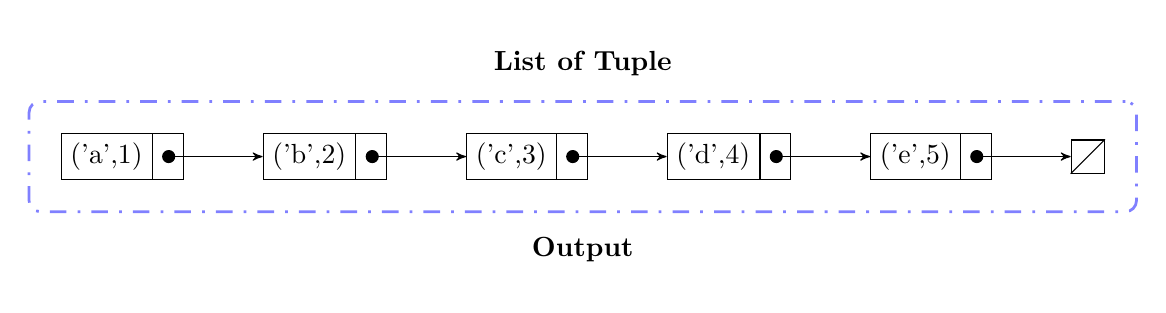
\begin{tikzpicture}[
            list/.style={
                rectangle split,
                rectangle split parts=2,
                draw,
                rectangle split horizontal
            },
            blue dotted/.style={
                draw=blue!50!white,
                line width=1pt,
                dash pattern=on 1pt off 4pt on 6pt off 4pt,
                inner sep=4mm,
                rectangle,
                rounded corners
            },
            node distance=2mm and 1cm]
                { [start chain=zip]
                    \node[list,on chain] (A1) {('a',1)};
                    \node[list,on chain] (A2) {('b',2)};
                    \node[list,on chain] (A3) {('c',3)};
                    \node[list,on chain] (A4) {('d',4)};
                    \node[list,on chain] (A5) {('e',5)};
                    \node[on chain,draw,inner sep=6pt] (A6) {};

                    \draw[*->] let \p1 = (A1.two), \p2 = (A1.center) in (\x1,\y2) -- (A2);
                    \draw[*->] let \p1 = (A2.two), \p2 = (A2.center) in (\x1,\y2) -- (A3);
                    \draw[*->] let \p1 = (A3.two), \p2 = (A3.center) in (\x1,\y2) -- (A4);
                    \draw[*->] let \p1 = (A4.two), \p2 = (A4.center) in (\x1,\y2) -- (A5);
                    \draw[*->] let \p1 = (A5.two), \p2 = (A5.center) in (\x1,\y2) -- (A6);
                    \draw (A6.north east) -- (A6.south west);

                    \node (zip dotted box) [blue dotted, fit = (A1) (A6)] {};
                    \node at (zip dotted box.north) [above, inner sep=3mm] {\textbf{List of Tuple}};
                    \node at (zip dotted box.south) [below, inner sep=3mm] {\textbf{Output}};
                }
            \end{tikzpicture}
        }
    \end{frame}

% FRAME:ZIP EXAMPLE
    \begin{frame}[fragile=singleslide]
        \frametitle{Zip (Lists and Tuples)}

        \begin{lstlisting}
// zip :: [a] -> [b] -> [(a,b)]        
        
lLetters = ['a', 'b', 'c', 'd']
lNumbers = [1, 2, 3, 4]

lZipped = zip lLetters lNumbers
// lZipped = [('a',1), ('b',2), ('c',3), ('d',4)]

lReversed = zip lNumbers lLetters
// lReversed = [(1,'a'), (2,'b'), (3,'c'), (4,'d')]
        \end{lstlisting}
    \end{frame}

% FRAME:LIST COMPREHENSION
    \begin{frame}[fragile=singleslide]
        \frametitle{List Comprehension}

        \begin{lstlisting}
powers = [ 2^x | x <- [1, 2, 3, 4, 5] ]
// powers = [2, 4, 8, 16, 32]
        \end{lstlisting}
        
        \begin{description}
            \item[|] "for every"
            \item[<-] "that is an element of"
        \end{description}
    \end{frame}

% FRAME:ON TO THE FIBS
    \begin{frame}[fragile=singleslide]
        \begin{figure}
            \centering
            
\includegraphics[scale=0.35]{./images/dalek-to-victory.jpg}
        \end{figure}
    \end{frame}

% FRAME:BUILDING A LIST
    \begin{frame}[fragile=singleslide]
        \frametitle{Begin with a List}

        \begin{figure}
            \begin{lstlisting}
fibs = [1, 1, 2, 3, 5]
            \end{lstlisting}
            \caption{Define the sequence explicitly.}
        \end{figure}
        \begin{figure}
            \begin{lstlisting}
fibs = 1 : 1 : [2, 3, 5]
            \end{lstlisting}
            \caption{Define only the first two fibs, then use some programmatic definition for the rest of the sequence.}
        \end{figure}
    \end{frame}

% FRAME:PLAYING WITH FUNCTIONS
    \begin{frame}[fragile=singleslide]
        \frametitle{Playing with Functions}

        \begin{figure}
            \begin{lstlisting}
fibs = 1 : 1 : [2, 3, 5, 8]
// fibs = [1, 1, 2, 3, 5, 8]

t = tail fibs
// t = [1, 2, 3, 5, 8]

z = zip fibs (tail fibs)
// z = [(1,1), (1,2), (2,3), (3,5), (5,8)]
            \end{lstlisting}
        \end{figure}
    \end{frame}

% FRAME:PLAYING WITH FUNCTIONS DIAGRAM
    \begin{frame}[fragile=singleslide]
        \frametitle{Playing with Functions}

        \adjustbox{scale=0.7} {
            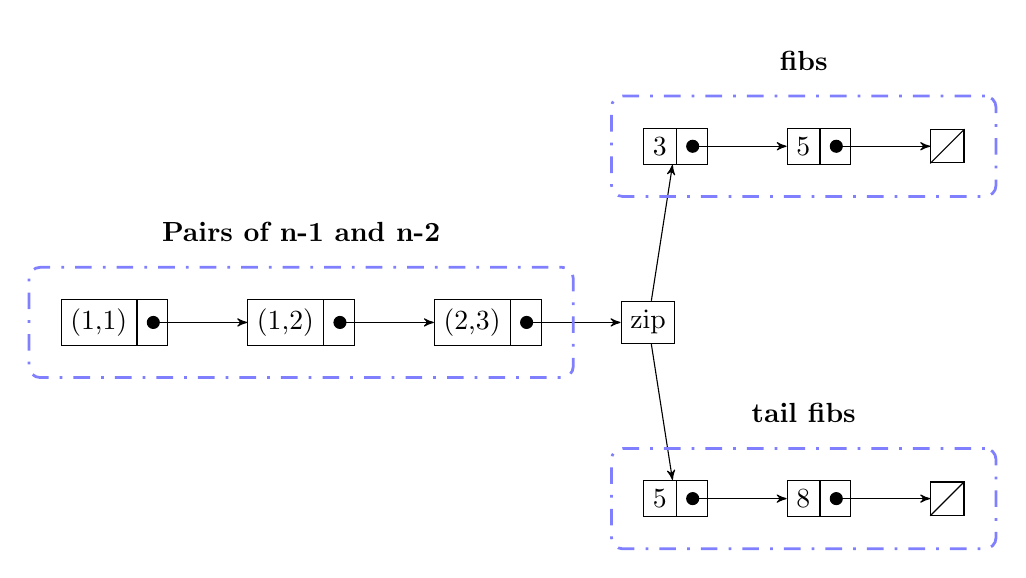
\begin{tikzpicture}[
            list/.style={
                rectangle split,
                rectangle split parts=2,
                draw,
                rectangle split horizontal
            },
            blue dotted/.style={
                draw=blue!50!white,
                line width=1pt,
                dash pattern=on 1pt off 4pt on 6pt off 4pt,
                inner sep=4mm,
                rectangle,
                rounded corners
            },
            node distance=2mm and 1cm]
                { [start chain=zip]
                    \node[list,on chain] (A1) {(1,1)};
                    \node[list,on chain] (A2) {(1,2)};
                    \node[list,on chain] (A3) {(2,3)};
                    \node[on chain,draw,rectangle] (zip) {zip};
                    { [start branch=letters going right]
                        \node[list,on chain, above=2cm] (B1) {3};
                        \node[list,on chain] (B2) {5};
                        \node[on chain,draw,inner sep=6pt] (B3) {};
                   
                        \draw (B3.north east) -- (B3.south west);
                        \draw[*->] let \p1 = (B1.two), \p2 = (B1.center) in (\x1,\y2) -- (B2);
                        \draw[*->] let \p1 = (B2.two), \p2 = (B2.center) in (\x1,\y2) -- (B3);
                        \draw[->] (zip) -- (B1);

                        \node (letters dotted box) [blue dotted, fit = (B1) (B3)] {};
                        \node at (letters dotted box.north) [above, inner sep=3mm] {\textbf{fibs}};
                    }
                    { [start branch=numbers going right]
                        \node[list,on chain, below=2cm] (C1) {5};
                        \node[list,on chain] (C2) {8};
                        \node[on chain,draw,inner sep=6pt] (C3) {};
                        
                        \draw (C3.north east) -- (C3.south west);
                        \draw[*->] let \p1 = (C1.two), \p2 = (C1.center) in (\x1,\y2) -- (C2);
                        \draw[*->] let \p1 = (C2.two), \p2 = (C2.center) in (\x1,\y2) -- (C3);
                        \draw[->] (zip) -- (C1);

                        \node (numbers dotted box) [blue dotted, fit = (C1) (C3)] {};
                        \node at (numbers dotted box.north) [above, inner sep=3mm] {\textbf{tail fibs}};
                    }

                    \draw[*->] let \p1 = (A1.two), \p2 = (A1.center) in (\x1,\y2) -- (A2);
                    \draw[*->] let \p1 = (A2.two), \p2 = (A2.center) in (\x1,\y2) -- (A3);
                    \draw[*->] let \p1 = (A3.two), \p2 = (A2.center) in (\x1,\y2) -- (zip);

                    \node (zip dotted box) [blue dotted, fit = (A1) (A3)] {};
                    \node at (zip dotted box.north) [above, inner sep=3mm] {\textbf{Pairs of n-1 and n-2}};
                }
            \end{tikzpicture}
        }
    \end{frame}

% FRAME:BUILD A COMPREHENSION
    \begin{frame}[fragile=singleslide]
        \frametitle{Building a Comprehension}

        \begin{figure}
            \begin{lstlisting}
fibs = 1 : 1 : [2, 3, 5, 8]

fibs2 = [ a + b | (a, b) <- zip fibs (tail fibs) ]
// fibs2 = [2, 3, 5, 8, 13]
            \end{lstlisting}
        \end{figure}

        \begin{itemize}
            \item[zip] The "zip fibs (tail fibs)" statement produces a list of tuples.
            \item[(a, b)] We bind each tuple to the names "a" and "b".
            \item[a + b] Each item in fibs2 is the sum of each tuple.
            \item Each element of fibs2 is the sum of "a" and "b", where "a" and "b" are elements of zipping together fibs and the tail of fibs.
        \end{itemize}
    \end{frame}

% FRAME:SECRET SAUCE
    \begin{frame}[fragile=singleslide]
        \frametitle{Lazy Evaluation (Haskell's secret sauce).}

        \begin{figure}
            \begin{lstlisting}
a = 2
b = 3 + 6

main = do
        putStrLn "Hello, World!"
        putStrLn (show (a + b))
            \end{lstlisting}
        \end{figure}
        \begin{itemize}
            \item[b] The value of 3 + 6 is not evaluated immediately.
            \item[putStrLn] This call prints to the screen, and requires full evaluation.
            \item[show] Converts arbitrary types to a string.
            \item The value of b is not evaluated until line 6 when it is printed to the console.
        \end{itemize}
    \end{frame}

% FRAME:MERGING FIBS AND FIBS2
    \begin{frame}[fragile=singleslide]
        \frametitle{Merging Fibs and Fibs2}

        \begin{figure}
            \begin{lstlisting}
fibs = 1 : 1 : [ a + b | (a, b) <- zip fibs (tail fibs) ]
            \end{lstlisting}
        \end{figure}

        \begin{columns}[c]
            \begin{column}[T]{5cm}
                Properties of Fib Sequence
                \begin{itemize}
                    \item Sequence is infinite.
                    \item Sequence is self-referencing.
                    \item Values grow exponentially.
                    \item Values are always positive.
                \end{itemize}
            \end{column}
            \begin{column}[T]{5cm}
                Properties of Haskell Implementation
                \begin{itemize}
                    \item fibs is and infinite sequence.
                    \item fibs references itself in its definition.
                    \item Integer values in Haskell support infinite precision.
                    \item It is impossible for a negative value to be produced.
                \end{itemize}
            \end{column}
        \end{columns}
    \end{frame}
\end{document}
